%%%%%%%%%%%%%%%%%%%%%%%%%%%%%%%%%%%%%%%%%%%%%%%%%%%%%%%%%%%%%%%%%%%%%%%%%%
%%%%%%%%%%%%%%%%%%%%%%%%%%%%%%%%%%%%%%%%%%%%%%%%%%%%%%%%%%%%%%%%%%%%%%%%%%
\clearpage{}
\section{Results}
\label{sec:results}
% ---- ---- ---- ---- ---- ---- ---- ---- ---- ---- ---- ---- ---- ---- ----
\par
The well-known formula for the extraction of  a cross section is:
\begin{equation}
\label{eq:xsec}
 \sigma = \frac{N^{\text{Sig}}}
               { A \, \epsilon \, {\cal{L}} }
\end{equation}
where $N^{\text{Sig}}$ is the number of extracted signal events,
$A$ is the signal acceptance corrected for the branching fraction,
$\epsilon$ is the efficiency for all requirements on 
the event selection, and ${\cal{L}}$ is the integrated luminosity.
Using the number of signal diboson events from 
table~\ref{table:FitTotalsAndComparisons} and efficiency $\times$ 
acceptance values from table~\ref{tab:signals}, we obtain the 
WW+WZ cross section values for each disjoint sub-sample as shown in 
table~\ref{tab:measuredCrossSection}
%%%%%%%%%%%%%%%%%%%%%%%%%%%%%
\begin{table}[h]
\begin{center}
  \begin{tabular}{l c}
    \hline  \hline
    Event category &  Measured cross section\\
    \hline
    $\mu jj$        &    $73.41 \pm 15.07$  pb\\
    $ejj$           &    $60.14 \pm 21.50$  pb\\   \hline 
    $\mu jj$,b-tag  &    $76.85 \pm 60.68$  pb\\
    $ejj$,b-tag     &    $22.71 \pm 49.27$  pb\\   \hline 
    Theory prediction~\cite{Campbell:2011bn} &  $65.6 \pm 2.2$ pb\\
    \hline  \hline
  \end{tabular}
\end{center}
\caption{\label{tab:measuredCrossSection}
The measured values of the sum of WW and WZ cross section in each disjoint sub-sample. 
The uncertainties include both statistical and systematic.}
\end{table}
%%%%%%%%%%%%%%%%%%%%%%%%%%%%%

Combining all four channels, we obtain:

WW+WZ cross section = 66.70 $\pm$ 11.74 pb.\\
[Breaking down the uncertainties: 66.70 $\pm$ 8.08 (stat) $\pm$ 8.52 (syst) pb]


We produce combined plots for electrons and muons in
Figs~\ref{fig:combinedNoBtag} and~\ref{fig:combinedWithBtag} for no $b$
tags and with $b$ tags, respectively.

\begin{figure}
\begin{center}
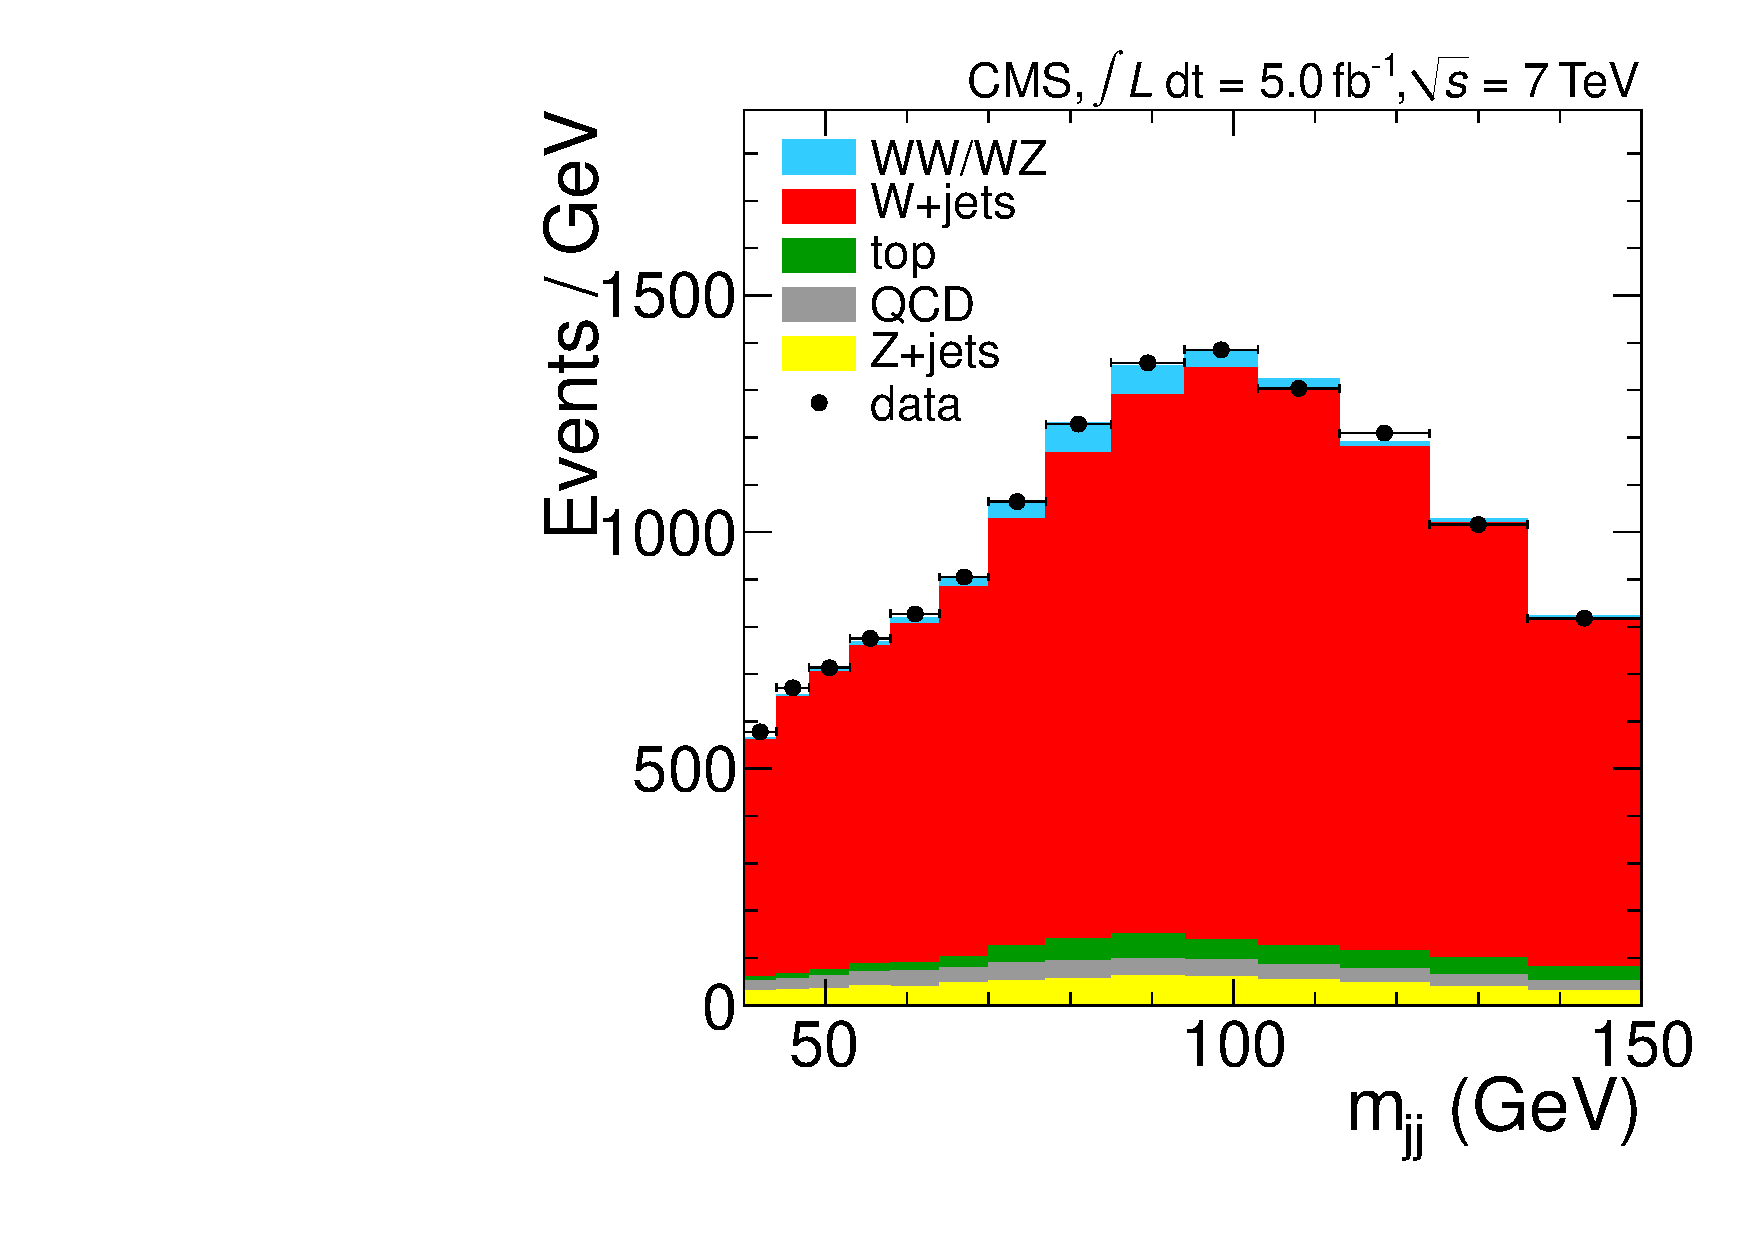
\includegraphics[width=0.45\textwidth]{figs/mjjfit_2jetsample/Diboson_Stacked_combined}
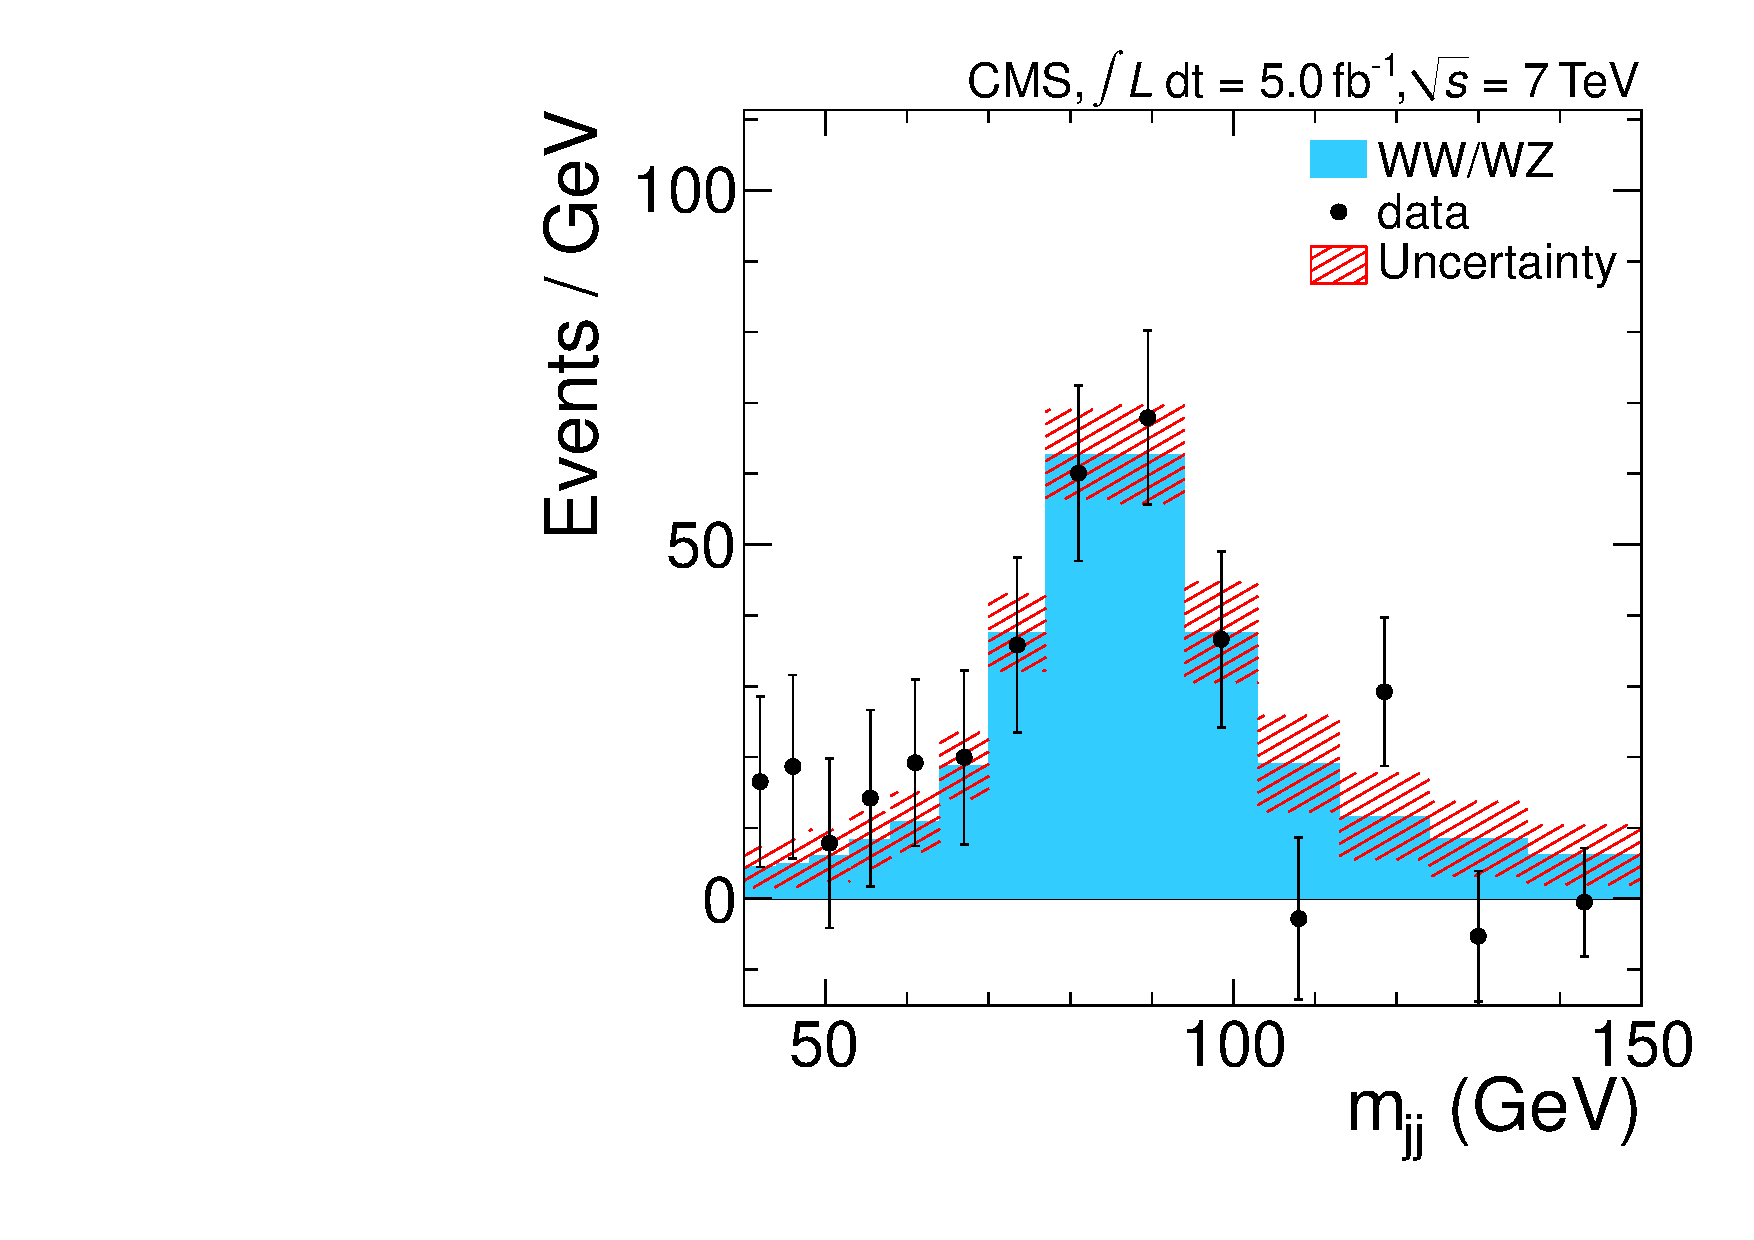
\includegraphics[width=0.45\textwidth]{figs/mjjfit_2jetsample/Diboson_Subtracted_combined}
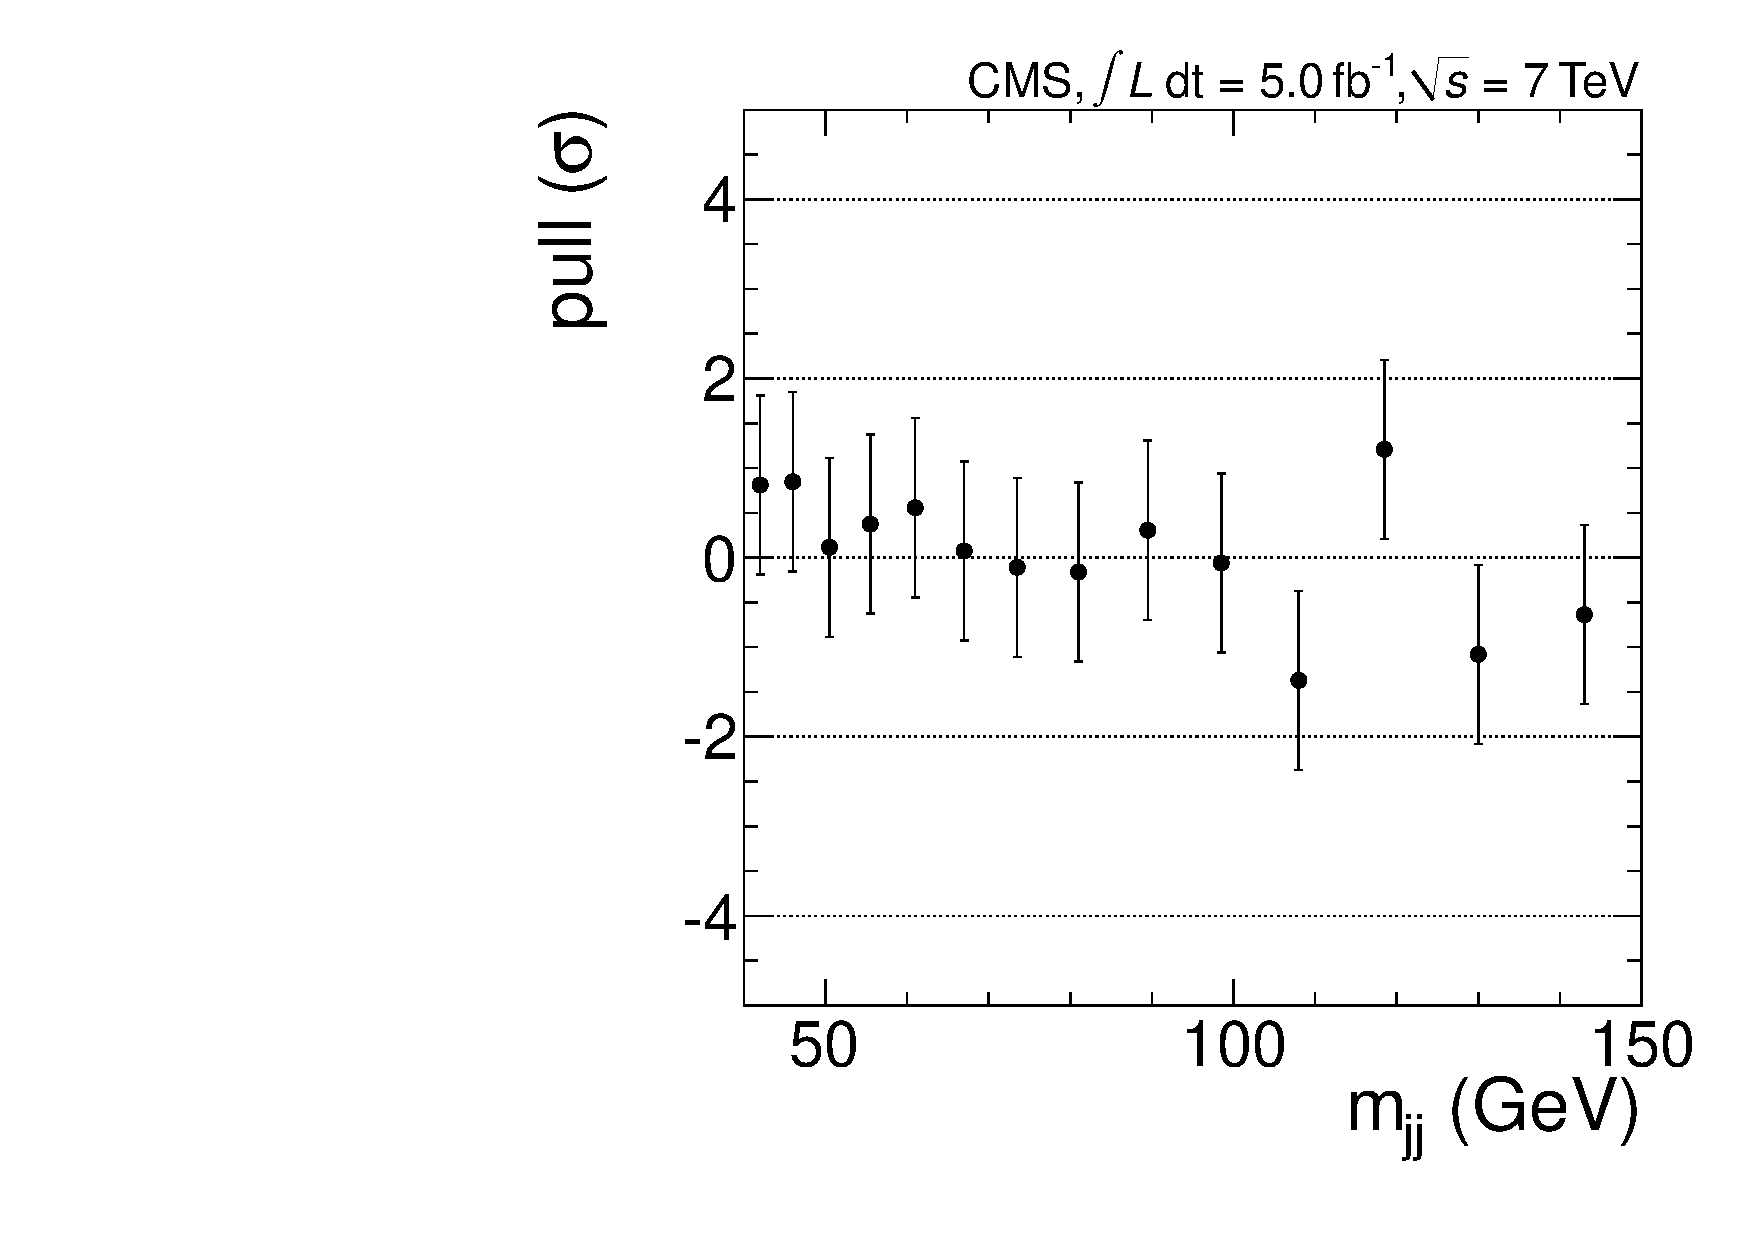
\includegraphics[width=0.45\textwidth]{figs/mjjfit_2jetsample/Diboson_Pull_combined}
\end{center}
\caption{Combined results of both muons and electrons without btags}
\label{fig:combinedNoBtag}
\end{figure}

\begin{figure}
\begin{center}
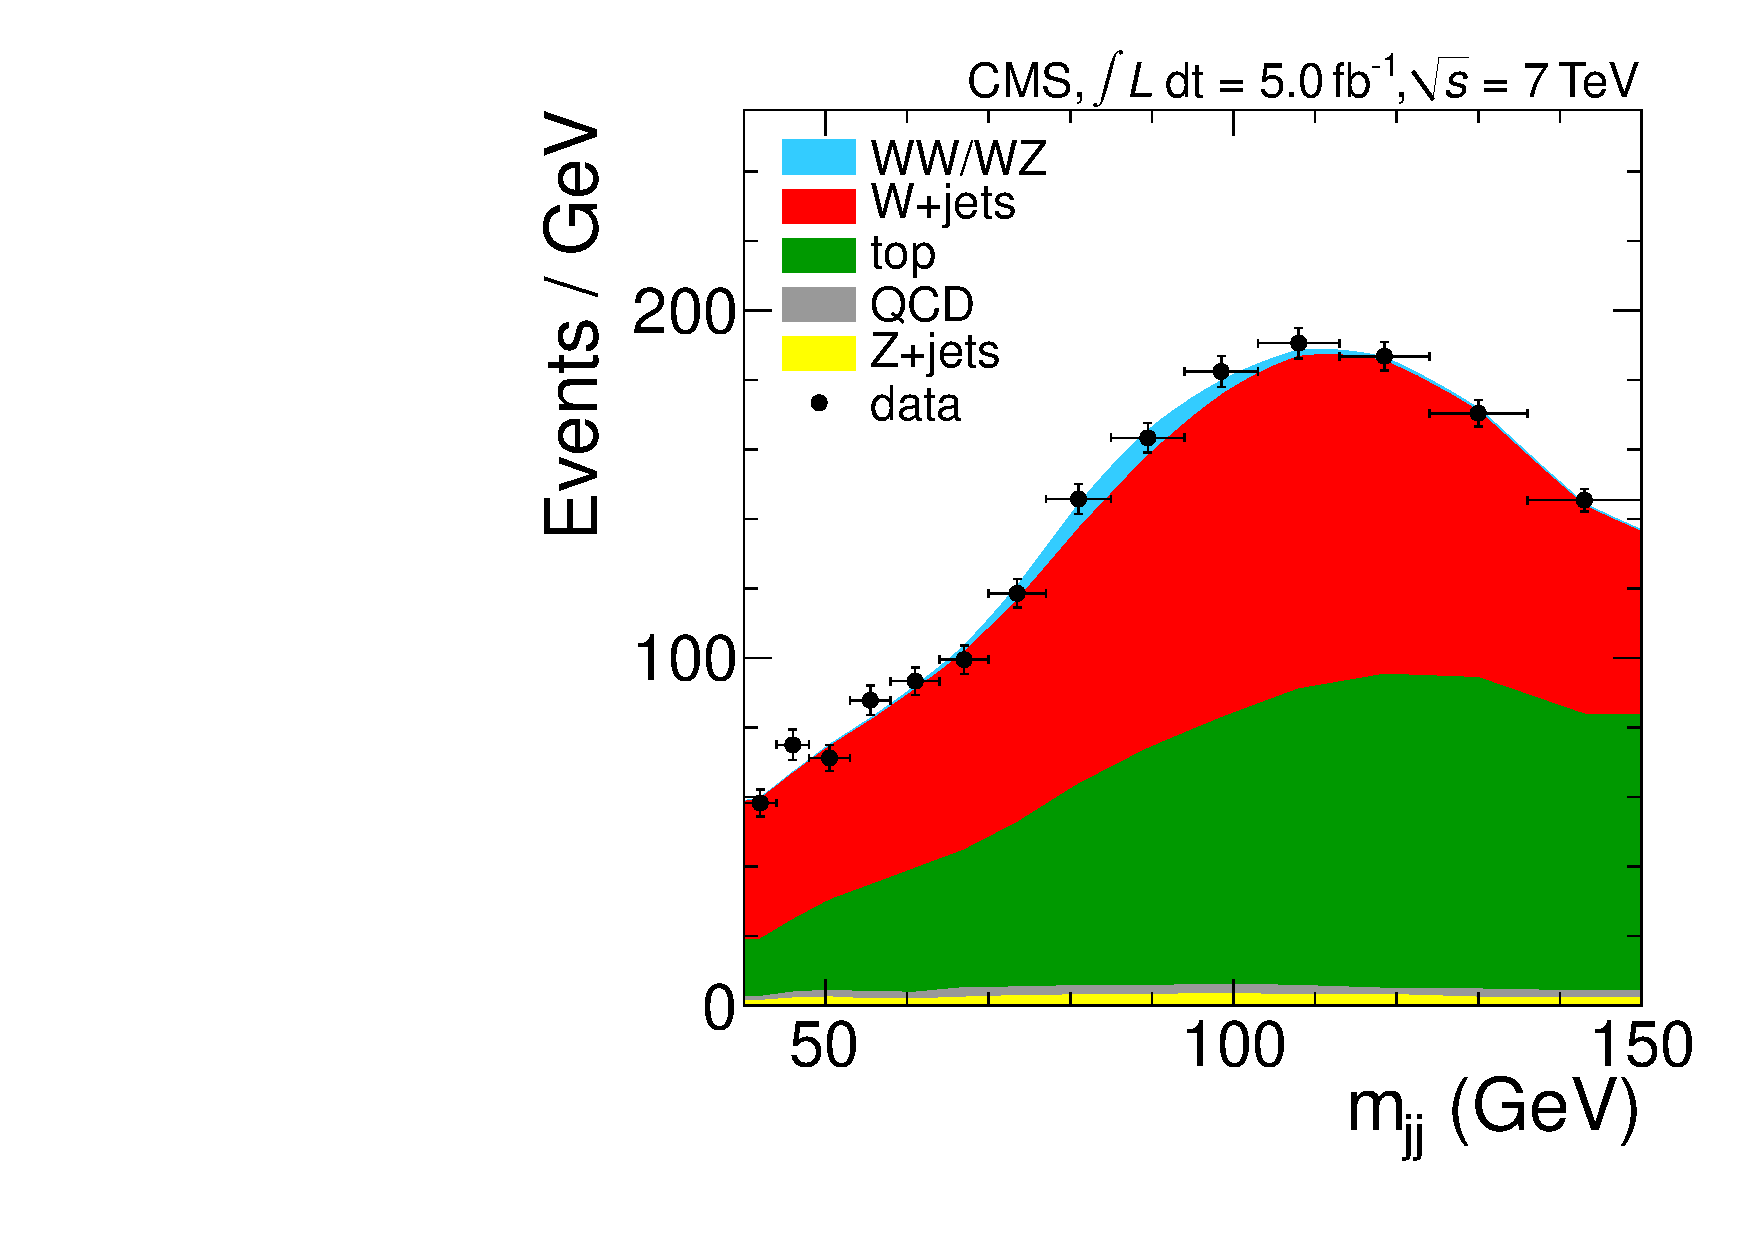
\includegraphics[width=0.45\textwidth]{figs/mjjfit_2jetsample/Diboson_btag_Stacked_combined}
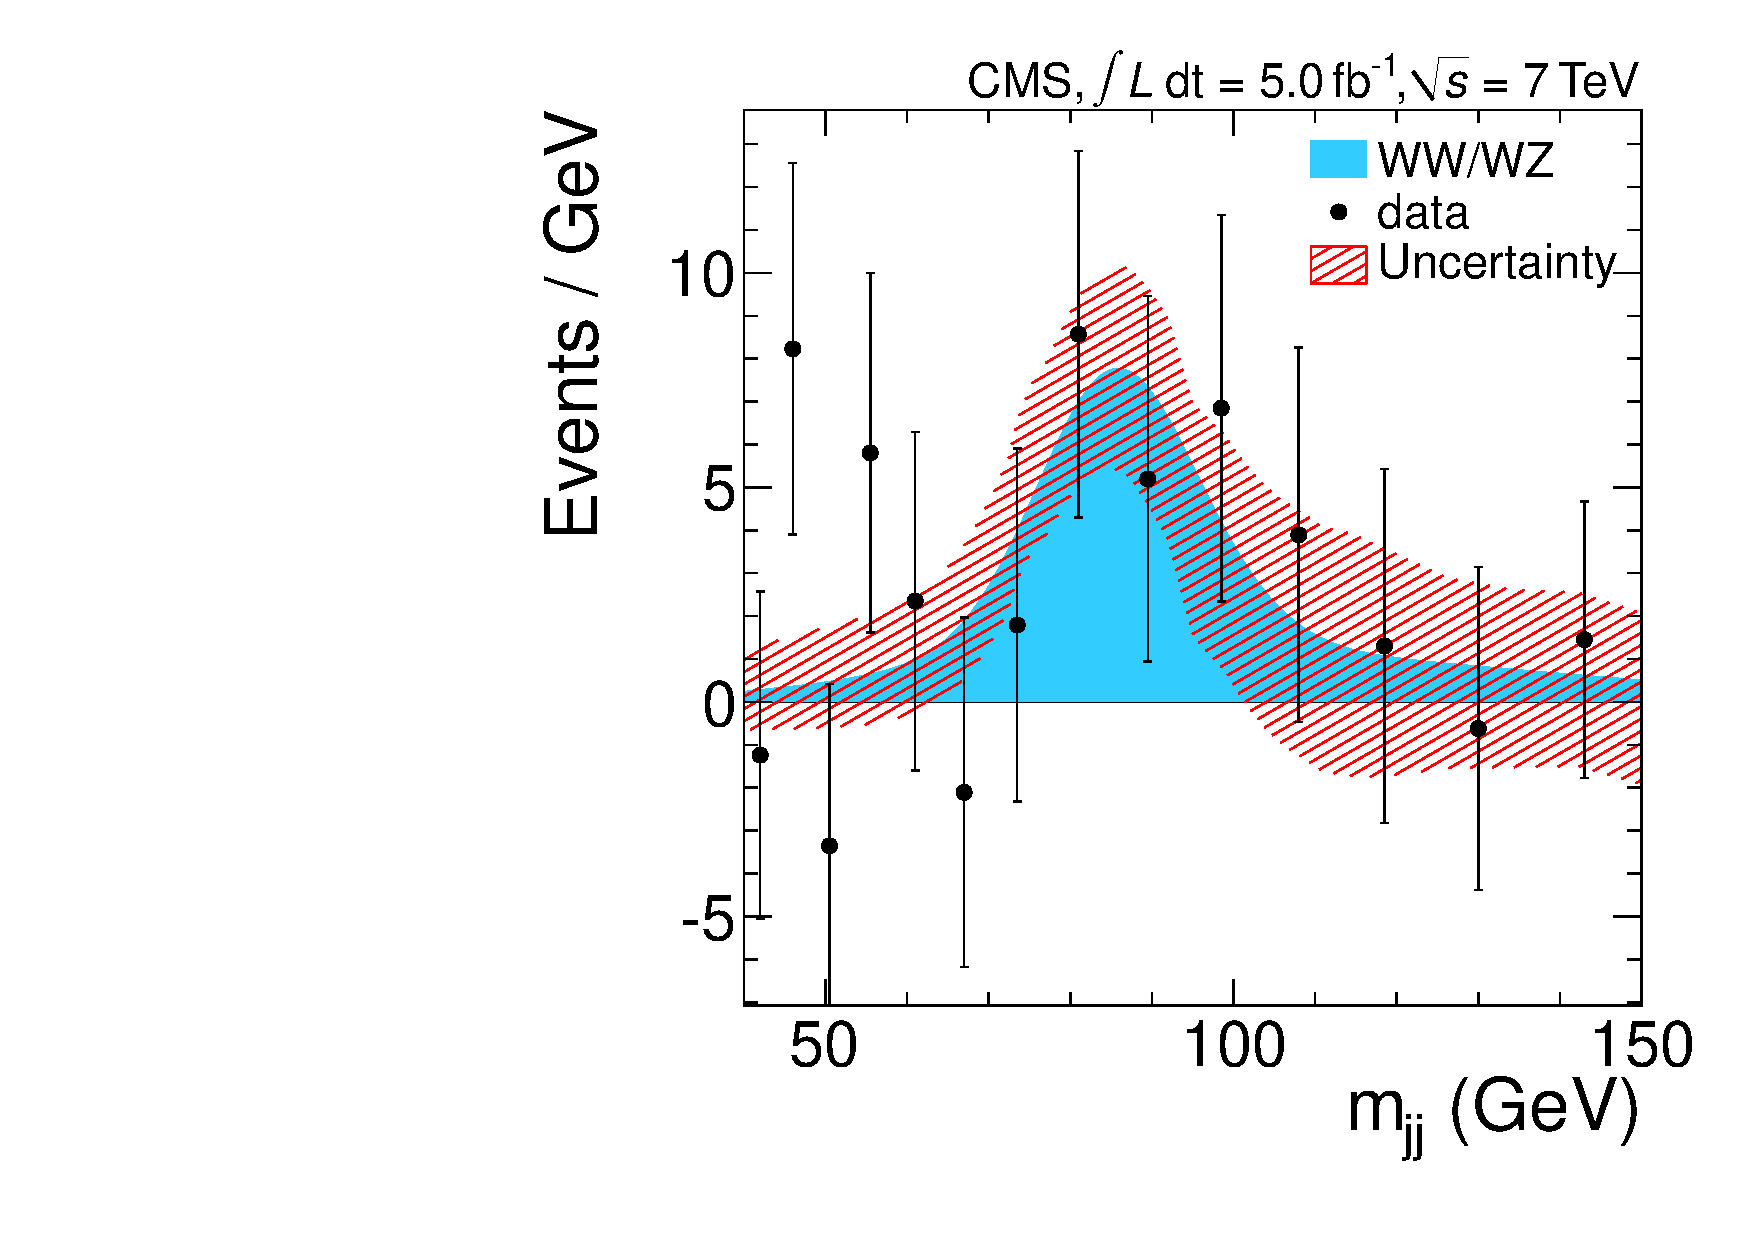
\includegraphics[width=0.45\textwidth]{figs/mjjfit_2jetsample/Diboson_btag_Subtracted_combined}
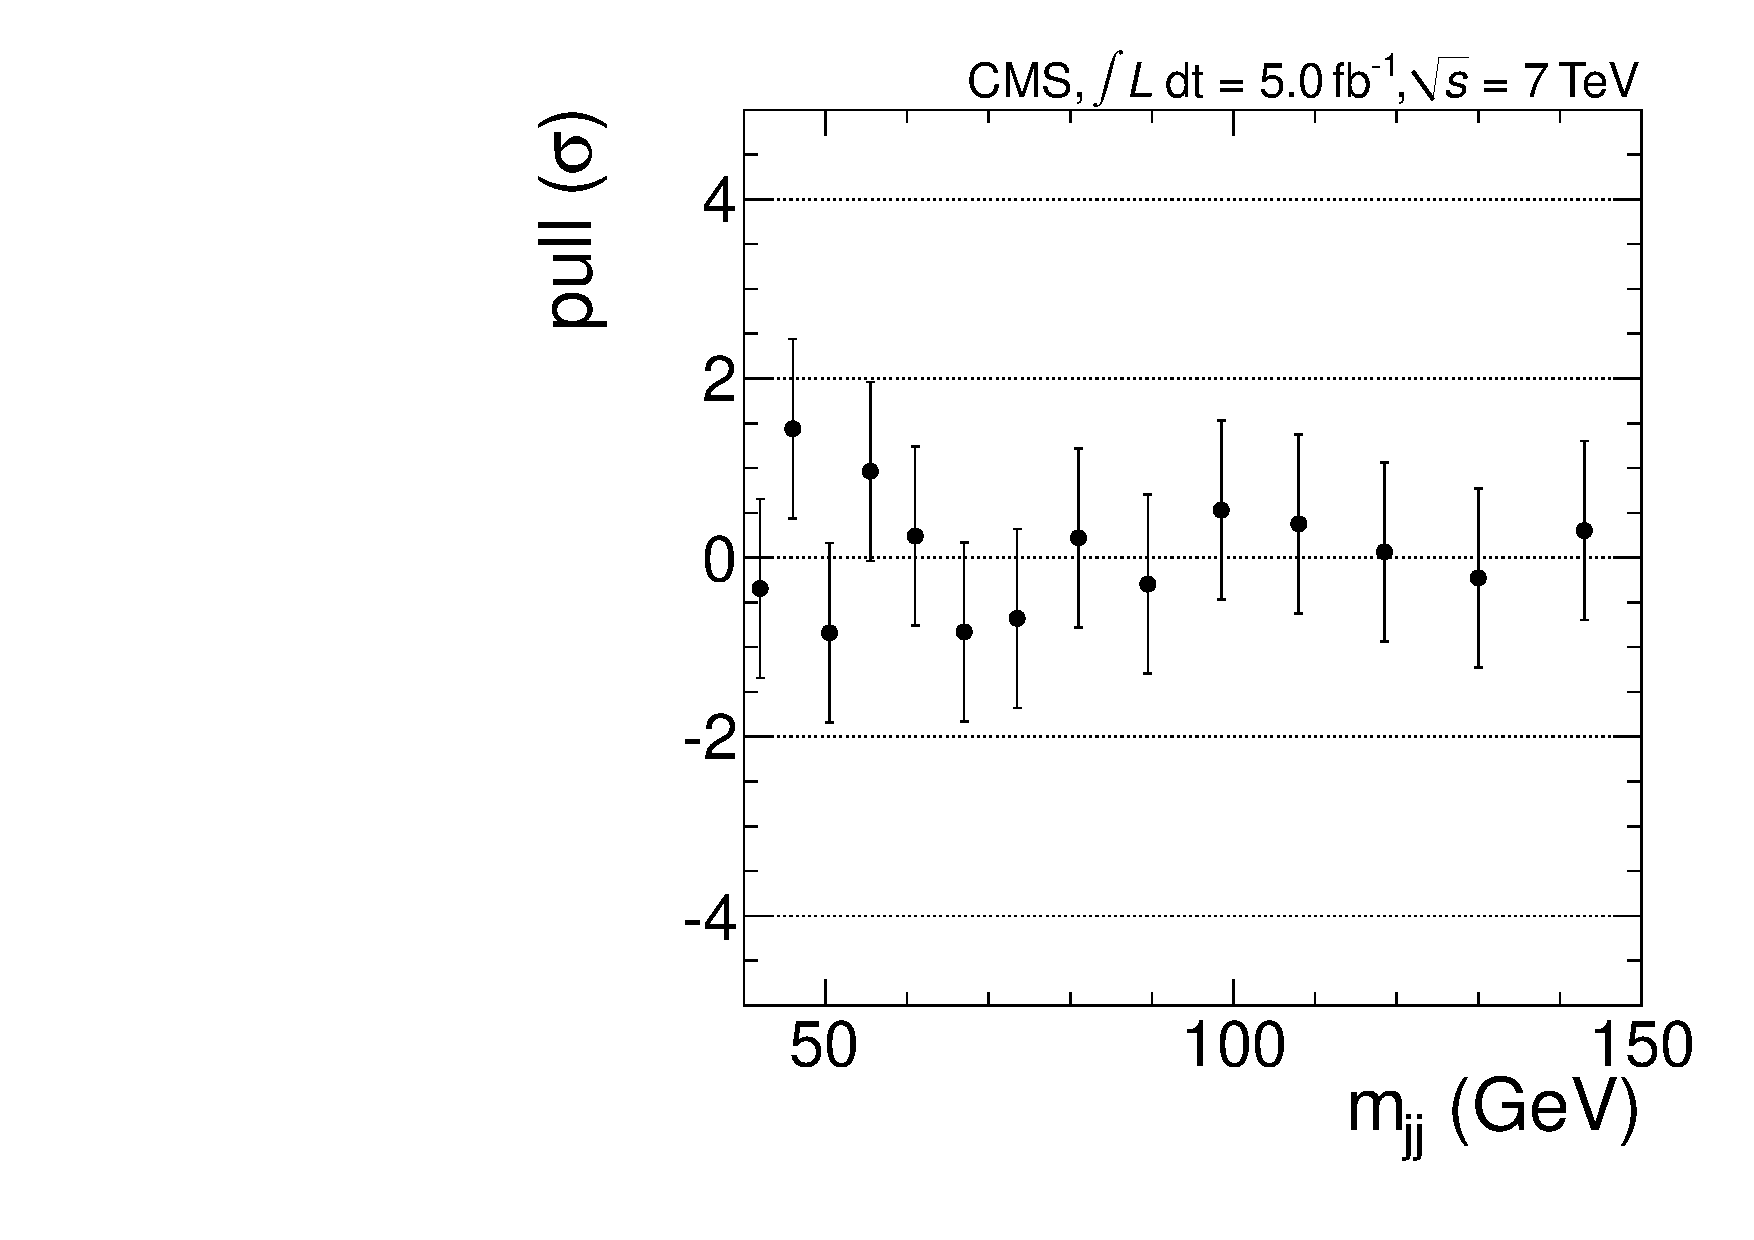
\includegraphics[width=0.45\textwidth]{figs/mjjfit_2jetsample/Diboson_btag_Pull_combined}
\end{center}
\caption{Combined results of both muons and electrons with btags}
\label{fig:combinedWithBtag}
\end{figure}


\subsection{Results including only non b-tag categories}
\label{sec:results2ch}
% ---- ---- ---- ---- ---- ---- ---- ---- ---- ---- ---- ---- ---- ---- ----
Including only non b-tag (both muon and electron) categories, we 
observe 2682 $\pm$ 339 (stat) $\pm$ 357 (syst) WW+WZ events, 
in agreement with the Standard Model expectation. 
This corresponds to a significance of $8.8~\sigma$ 
($7.8~\sigma$ in muon data and $4.4~\sigma$ in electron data) 
when computed using a simple likelihood 
ratio where the nuisance parameters are fixed to their nominal fit 
values in case of the null hypothesis. 
Using the profile likelihood ratio, where the nuisance parameters are 
allowed to vary also for the null hypothesis, the significance 
becomes $4.34~\sigma$ ($4.31~\sigma$ in muon data 
and $1.60~\sigma$ in electron data).


Combining results of muon and electron non b-tag categories, we obtain
the following result for cross section:
$\sigma = 68.89 \pm 8.71 \text{(stat)} \pm 9.70 \text{(syst)}  \pm 1.52 \text{(lumi)}$~pb, 
which is in agreement with the NLO prediction 
$65.6 \pm 2.2$~pb that includes $gg\to\text{WW}$ contribution.
